
To concentrate on your research, consider organizing your figures
first.  Build the document around your figures, and you will be able
to concentrate on the story of your contribution---not the work that
has gone on before.  

To organizing your figures, it is helpful to define them in a
common file.  See {\em myFigures.tex} depicted in
Figure~\ref{fig:myFigures} and stored in the Preamble subdirectory.
In this way, you may:
    \begin{itemize}
      \item Readily write new figures using earlier examples. 
      
      \item  Isolate code and minimize the risk of introducing bugs in the
      final editing process.  Moving around one line of
      code is easy and safe.
      
      \item Standardize figures without having to locate them 
      throughout the document.
      
      \item  Reuse figures in other papers.  $\leftarrow$ The best reason!
    \end{itemize}
        
\noindent In {\em myFigures.tex}, use {\bf
$\backslash${newcommand}} to define a command for each figure as
below:

{\vspace{-.30in}}
{\singlespace
\begin{verbatim}
\newcommand{\figmyFigures}{
    \begin{figure}[htbp]
        \begin{center}
             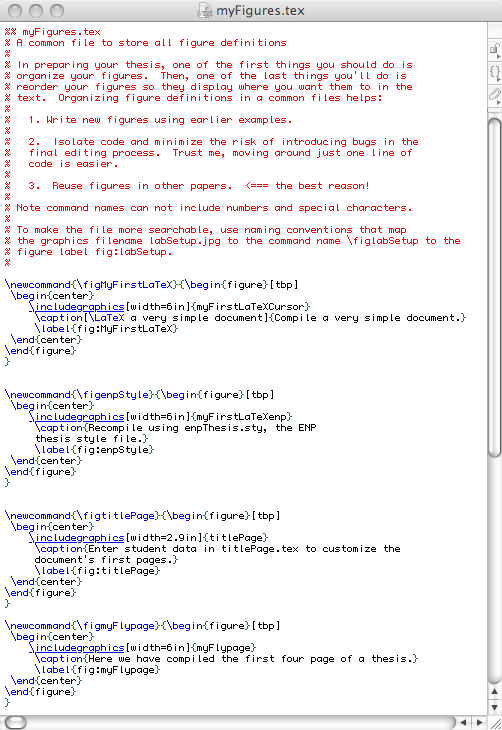
\includegraphics[width=6in]{myFigures}
             \caption{A sample tex file where figures are defined.}
             \label{fig:myFigures}
        \end{center}
    \end{figure}
}
\end{verbatim}}
    
\noindent For a command, chose a naming convention that
intuitively links the command to the graphic file and the figure
label.  For example, above we have defined a command {\bf
$\backslash${figmyFigures}} to position a figure containing graphic
myFigures.png.  Note command names cannot include numbers or special
characters.


